% Two-layer forward propagation demo diagram
\documentclass[tikz,border=8pt]{standalone}
\usepackage{tikz}
\usetikzlibrary{positioning,fit,backgrounds,arrows.meta}

\tikzset{
  every picture/.append style={
    execute at end picture={
      \begin{scope}[on background layer]
        \draw[rounded corners=6pt, line width=0.8pt, gray!60]
          ([xshift=-6pt,yshift=-6pt]current bounding box.south west) rectangle
          ([xshift=6pt,yshift=6pt]current bounding box.north east);
      \end{scope}
    }
  }
}

\begin{document}
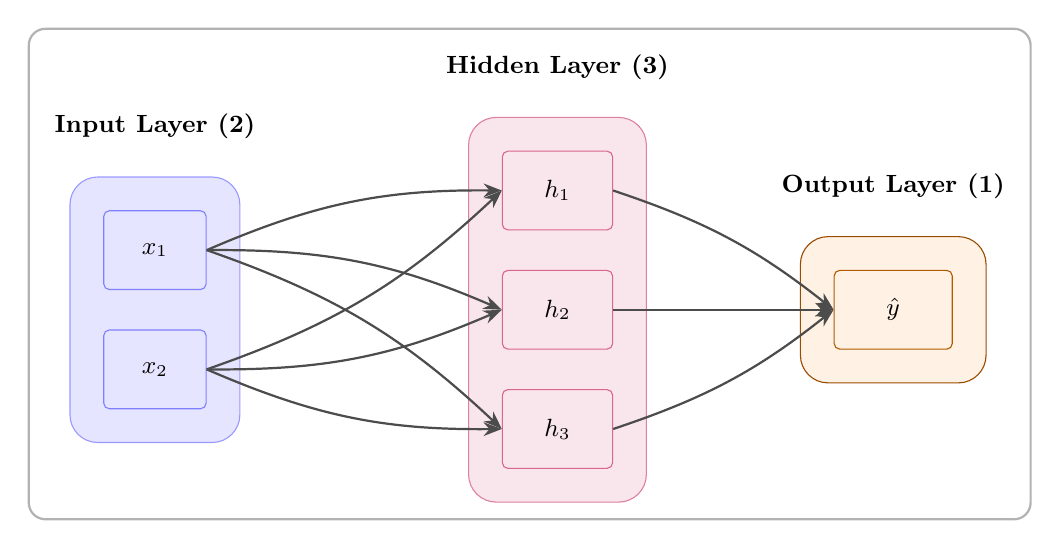
\begin{tikzpicture}[
        font=\small,
        node distance=1.4cm,
        >=Stealth,
        input/.style={draw=blue!50, rounded corners=2pt, minimum width=1.3cm, minimum height=1cm, fill=blue!10},
        hidden/.style={draw=purple!60, rounded corners=2pt, minimum width=1.4cm, minimum height=1cm, fill=purple!10},
        output/.style={draw=orange!70!black, rounded corners=2pt, minimum width=1.5cm, minimum height=1cm, fill=orange!10},
        arrow/.style={->, thick, draw=black!70},
    ]

    % 输入层
    \matrix[column sep=0.8cm, row sep=0.5cm] (inputs) {
        \node[input] (x1) {$x_1$}; \\
        \node[input] (x2) {$x_2$}; \\
    };
    % 隐藏层
    \matrix[column sep=1.2cm, row sep=0.5cm, right=3.5cm of inputs] (hidden) {
        \node[hidden] (h1) {$h_1$}; \\
        \node[hidden] (h2) {$h_2$}; \\
        \node[hidden] (h3) {$h_3$}; \\
    };
    % 输出层
    \node[output, right=2.8cm of h2] (yhat) {$\hat{y}$};

    % 连接:输入 -> 隐藏
    \foreach \h in {1,2,3} {
            \draw[arrow, bend left=12]  (x1.east) to (h\h.west);
            \draw[arrow, bend right=12] (x2.east) to (h\h.west);
        }

    % 连接:隐藏 -> 输出
    \draw[arrow, bend left=10] (h1.east) to (yhat.west);
    \draw[arrow] (h2.east) to (yhat.west);
    \draw[arrow, bend right=10] (h3.east) to (yhat.west);

    % 背景层区域
    \begin{scope}[on background layer]
        \node[draw=blue!40, fill=blue!10, rounded corners=10pt, inner sep=12pt, fit=(x1)(x2)] (inputbox) {};
        \node[draw=purple!50, fill=purple!10, rounded corners=10pt, inner sep=12pt, fit=(h1)(h2)(h3)] (hiddenbox) {};
        \node[draw=orange!60!black, fill=orange!10, rounded corners=10pt, inner sep=12pt, fit=(yhat)] (outputbox) {};
    \end{scope}

    % 分层标签
    \node[font=\bfseries\small, above=0.35cm of inputbox.north] {Input Layer (2)};
    \node[font=\bfseries\small, above=0.35cm of hiddenbox.north] {Hidden Layer (3)};
    \node[font=\bfseries\small, above=0.35cm of outputbox.north] {Output Layer (1)};

\end{tikzpicture}
\end{document}
